\documentclass{beamer}
\usepackage[utf8]{inputenc}
\usepackage{tikz}
\usetikzlibrary{arrows.meta}
\tikzset{>={Latex[width=2mm,length=2mm]},
  base/.style = {
    rectangle, rounded corners, draw=black,
    minimum height=1cm, text centered, font=\sffamily
  },
  process/.style = {
    base, minimum width=2.5cm, fill=orange!15,
    font=\ttfamily
  },
}

\graphicspath{{./img/},{../2021_05/img/},{../2020_03/img/}}
\DeclareGraphicsExtensions{.png,.jpg,.pdf}

\usepackage{hyperref}
\hypersetup{colorlinks,urlcolor=blue!50!black,linkcolor=red}

\usepackage{fontawesome}
\usepackage{listings}

\title{\small Máster en Sistemas Electrónicos Avanzados (MSEA)\\\Large Co-simulación y verificación funcional con\\VHDL, C/C++ y Python/m\\{\small $\{$control$\}$}}
\author{Unai Martinez Corral\\\href{mailto:unai.martinezcorral@ehu.eus}{\faEnvelope~unai.martinezcorral@ehu.eus}\\\href{https://orcid.org/0000-0003-1752-9181}{\faGlobe~ORCID} ~\href{https://github.com/umarcor}{\faGithub~umarcor} ~\href{https://gitlab.com/umarcor}{\faGitlab~umarcor}}
\institute{Escuela de Ingeniería de Bilbao\\Universidad del País Vasco/Euskal Herriko Unibertsitatea (UPV/EHU)}
\date{2022/05}

\begin{document}

\frame{\titlepage}

\begin{frame}
\frametitle{System under test}
\centering
\vfill
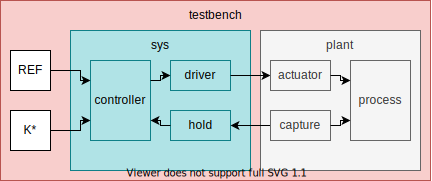
\includegraphics[width=\linewidth]{control.pdf}
\vfill
\end{frame}

\begin{frame}
\frametitle{Sharing data through files (text, CSV, binary, etc.)}
\centering
\vfill
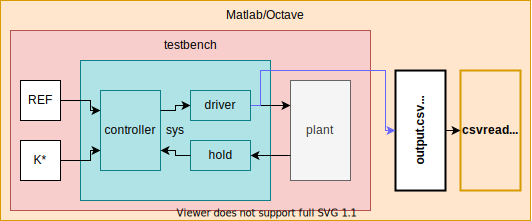
\includegraphics[width=\linewidth]{control_file.pdf}
\vfill
\end{frame}

\begin{frame}
\frametitle{Sharing data through cosimulation (compiled)}
\centering
\vfill
\includegraphics[width=\linewidth]{control_mkoctfile.pdf}
\vfill
\end{frame}

\begin{frame}
\frametitle{Sharing data through cosimulation (dynamic loading)}
\centering
\vfill
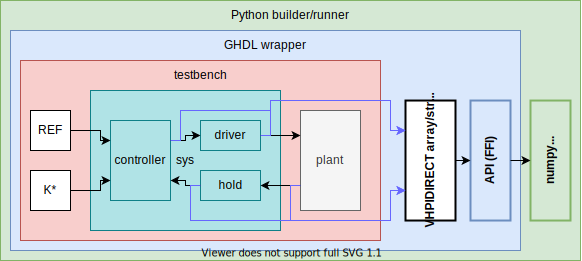
\includegraphics[width=\linewidth]{control_py.pdf}
\vfill
\end{frame}

\begin{frame}
\frametitle{Minimal System on Chip}
\centering
\vfill
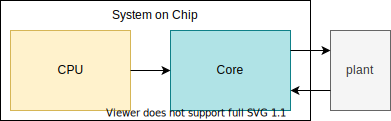
\includegraphics[width=\linewidth]{control_soc.pdf}
\vfill
\end{frame}

\begin{frame}
\frametitle{System on Chip (SoC)}
\centering
\vfill
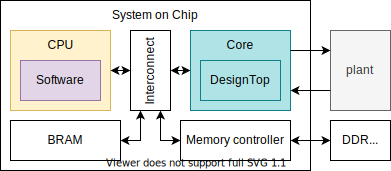
\includegraphics[width=\linewidth]{control_socmem.pdf}
\vfill
\end{frame}

\begin{frame}
\frametitle{NEORV32 SoC}
\centering
\vfill
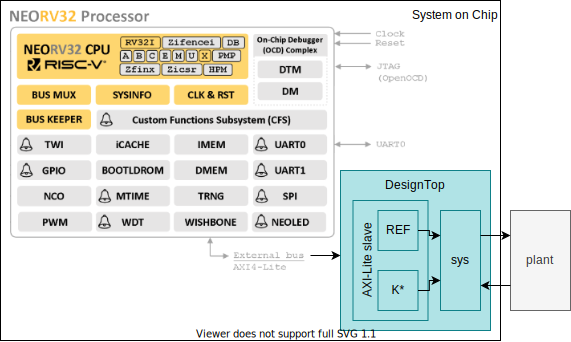
\includegraphics[width=\linewidth]{control_neorv32.pdf}
\vfill
\end{frame}

\begin{frame}
\frametitle{Exercise}
\centering
\vfill
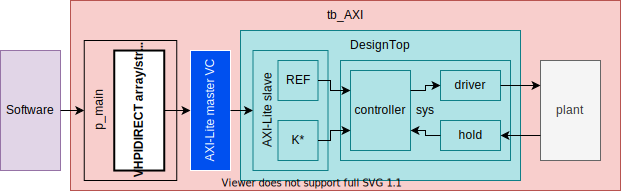
\includegraphics[width=\linewidth]{control_axilite.pdf}
\vfill
\end{frame}

\begin{frame}
\frametitle{Assignment}
\centering
\vfill
\includegraphics[width=\linewidth]{control_assignment.pdf}
\vfill
\end{frame}

\end{document}
